%DO NOT MESS AROUND WITH THE CODE ON THIS PAGE UNLESS YOU %REALLY KNOW WHAT YOU ARE DOING
\chapter*{Structuring the Project}
\addcontentsline{toc}{chapter}{Structuring the Project}
\noindent There are two main criteria which are interdependent, the Work Breakdown Structure (WBS) and the Organisational Breakdown Structure (OBS). Together, these help in the formation of the Responsibility Matrix (RM) for a project.

\section{ Work Breakdown Structure } \label{ Work Breakdown Structure }
\noindent The top level represents the final deliverable or project. Sub-deliverables contain work packages that are assigned to a department or unit. The WBS of the project consists of three levels, each hierarchy is identified with separate colours and is as shown in Figure 2.

\noindent The work breakdown structure has a number of benefits in addition to defining and organizing the project work. A project budget can be allocated to the top levels of the work breakdown structure, and department budgets can be quickly calculated based on the each project's work breakdown structure. By allocating time and cost estimates to specific sections of the work breakdown structure, a project schedule and budget can be quickly developed. As the project executes, specific sections of the work breakdown structure can be tracked to identify project cost performance and identify issues and problem areas in the project organization.

\begin{figure}[H]
\centering
{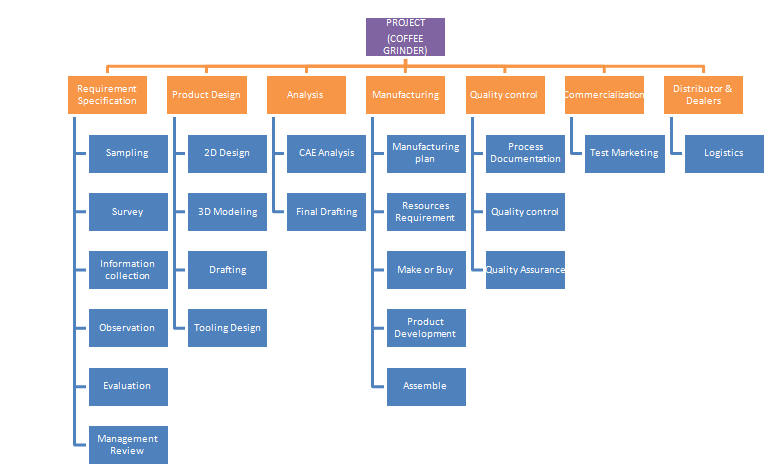
\includegraphics[scale=0.8]{wbs.png}}
\caption{Work Breakdown Structure}
\end{figure}

\section{ Responsibility Matrix } \label{ Responsibility Matrix }
\noindent Responsibility Matrix informs the organisation about its employees workload as it shows which role(s) are assigned to each person. For example, the organisation can see if someone has been placed in the responsible role too many times or not. In other words, does this person have a lot or a too few tasks to complete. That way, the organisation knows whether someone has too many or could take-on more responsibilities.

\noindent  Figure 3 shows the responsibility matrix for this project. R in the Figure 3 stands for responsible which means the resource responsible for completing the work to achieve a task or make a decision. Only one resource is responsible for a task, but additional resource(s) are delegated to assist in completing the work (supported), which are marked as S.

\begin{figure}[H]
\centering
{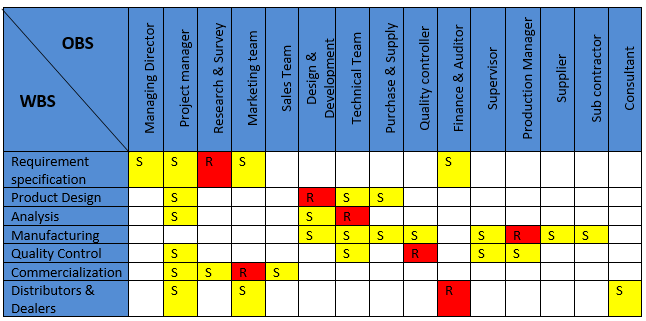
\includegraphics[scale=1.0]{matrix.png}}
\caption{Responsibility Matrix}
\end{figure}

